%!TEX root=../main.tex

In recent years, the analysis of multivariate functional data has become a popular method with applications in several fields. Functional principal component analysis (FPCA) is an extension of principal components analysis to functional data. FPCA has become a prevalent tool in FDA due to its abililty to convert infinite-dimensional functional data into finite-dimensional vectors of random scores. Multivariate functional principal components analysis (MFPCA) is the extension of FPCA to multivariate functional data. It allows to identify and visalize the main sources of variation in the data. 

We discuss the estimation of the number of components method in the recently published paper titled ``Multivariate Functional Principal Component Analysis for Data Observed on Different (Dimensional) Domains'' by \cite{happMultivariateFunctionalPrincipal2018a}.

In \cite{happMultivariateFunctionalPrincipal2018a}, the authors first estimate the principal components for each individual feature and combine them to derive the multivariate components. So, they chose a number of components for each individual feature and then use only these ones to compute the multivariate components. Let $K_p$ be the number of components retained for the $p$th feature. As the univariate components are concatenated to estimated the multivariate components, the number of multivariate components that can be estimated is $\sum_p K_p$. We however claim that only $\min_p K_p$ can only be accurately estimated.

The estimation of the number of components can also be done using the percentage of variance explained. 

We are interested by the estimation of the eigenvalues of functional datasets. Simulations are the same as the first setting in \cite{happMultivariateFunctionalPrincipal2018a}. The accuracy of the resulting estimates $\widehat{\lambda}_j$ is measured by the relative errors $\text{Err}(\widehat{\lambda}_j)  = (\lambda_j - \widehat{\lambda}_j)^2 / \lambda^2_j$.


\begin{figure}
     \centering
    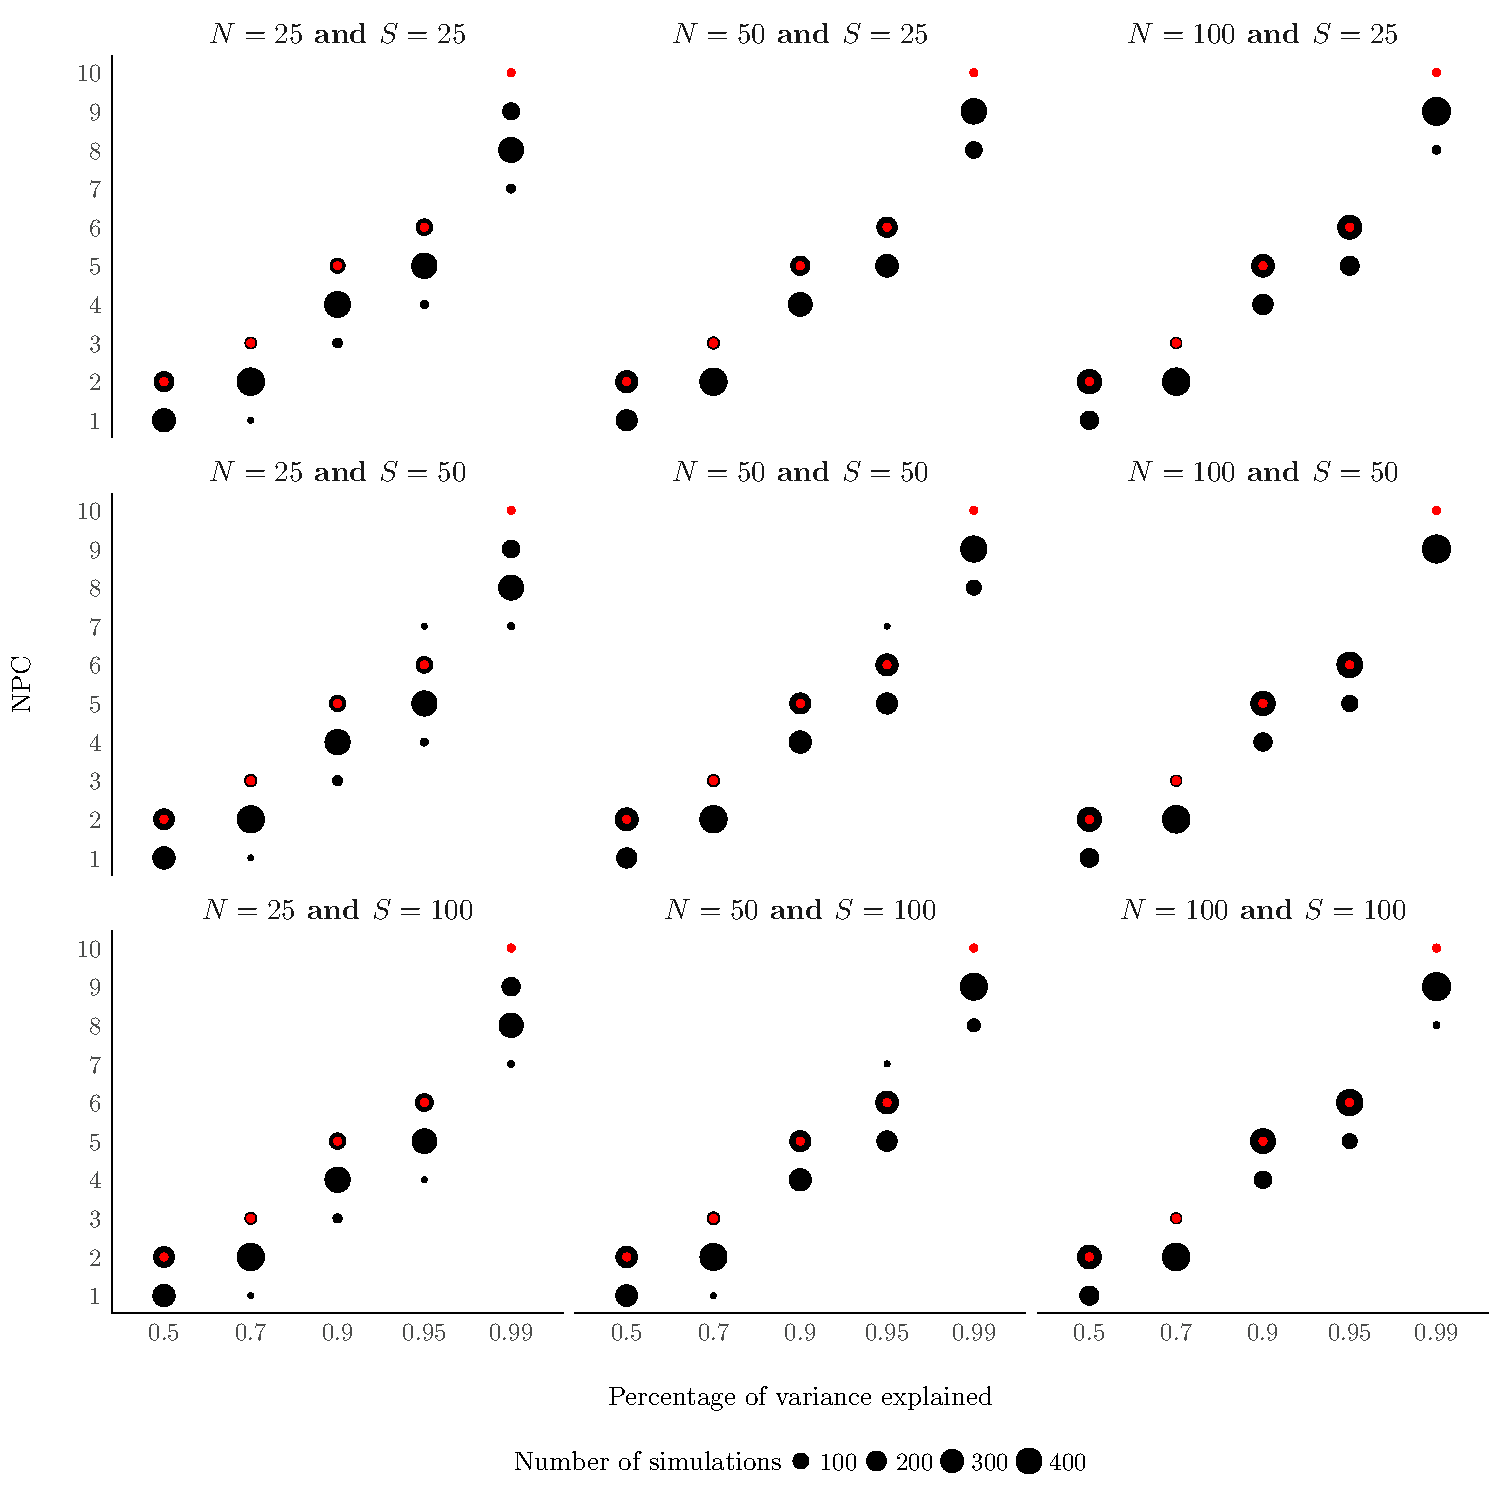
\includegraphics[width=0.95\textwidth]{figures/npc_estim.pdf}
    \caption{$N$ is the number of observations, $M$ is the number of sampling points per curve.}
    \label{fig:npc_estim}
\end{figure}

\begin{figure}
     \centering
    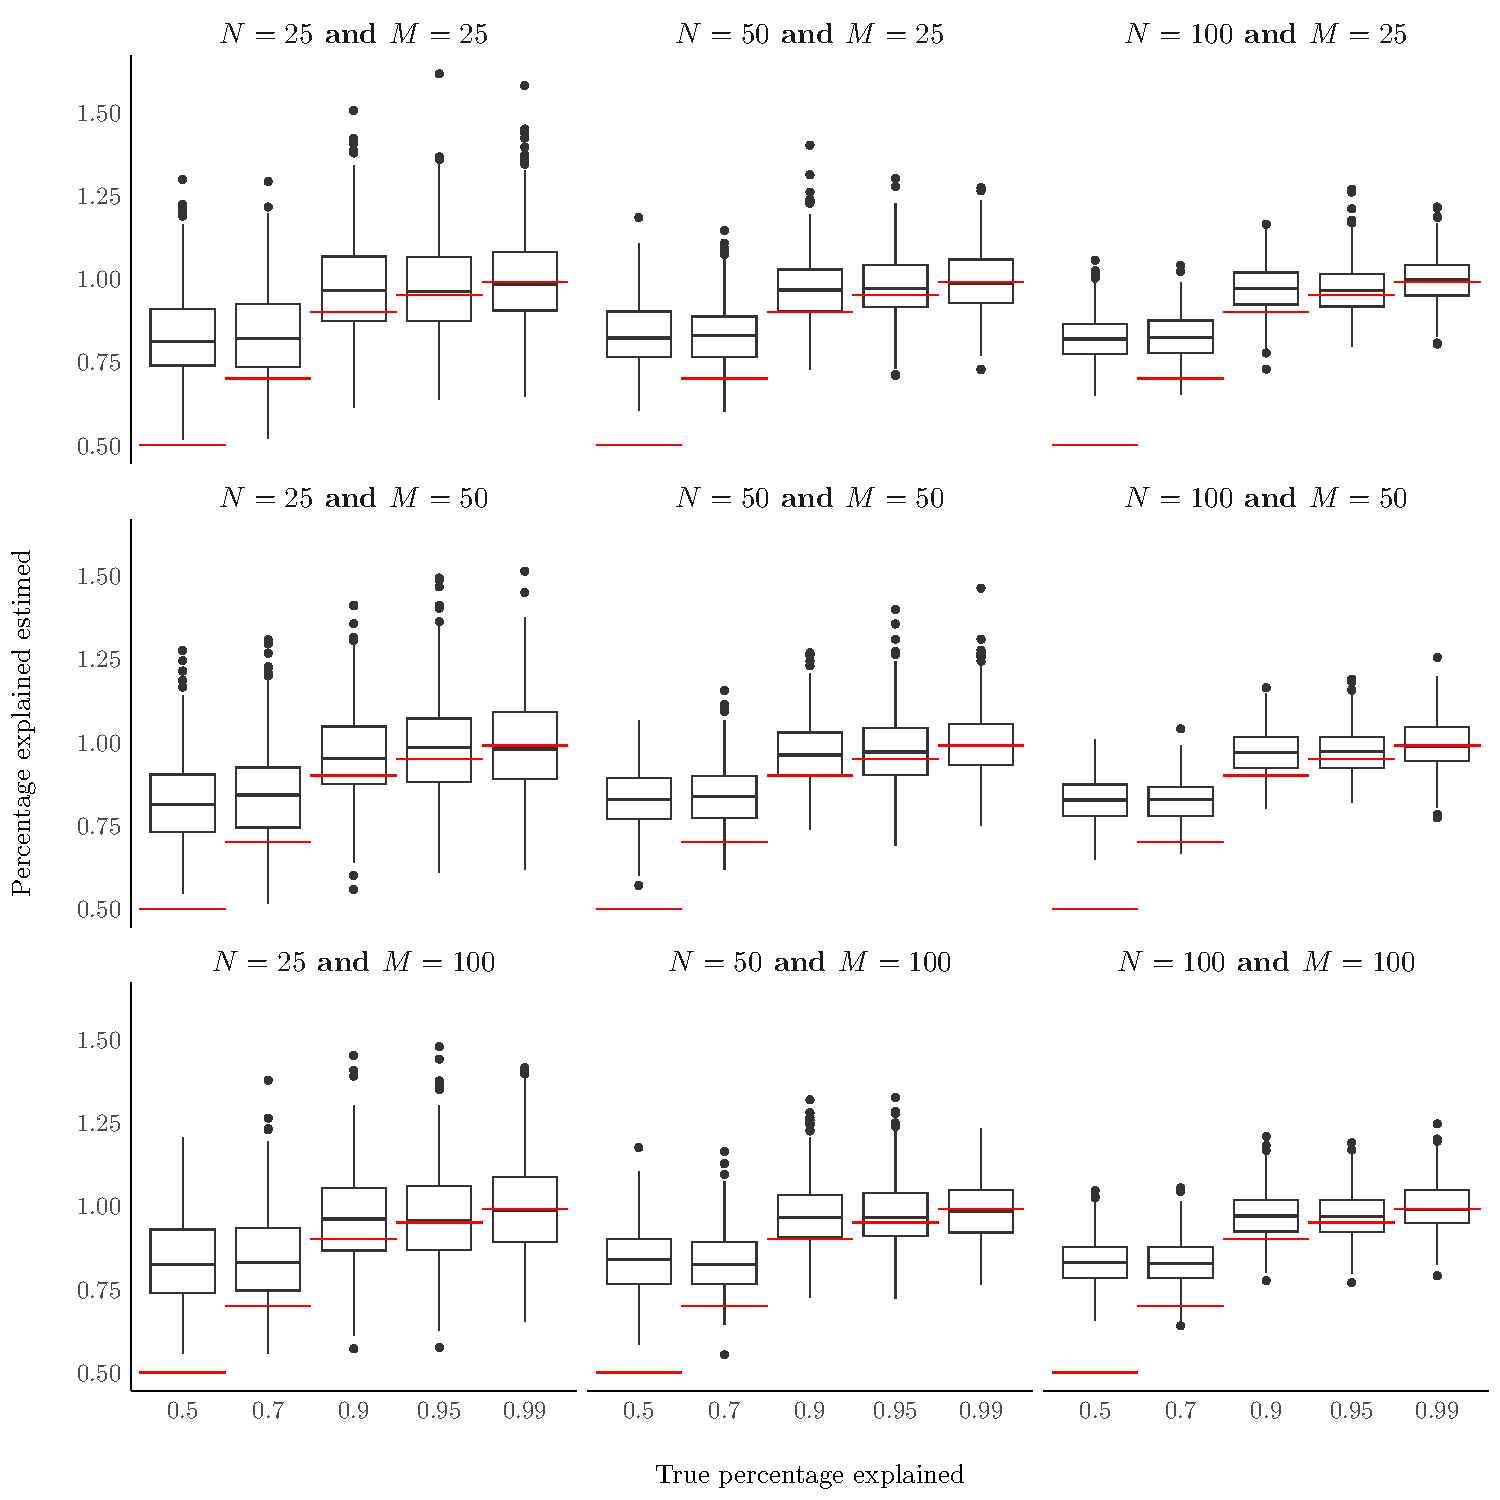
\includegraphics[width=0.95\textwidth]{figures/pct_estim.pdf}
    \caption{$N$ is the number of observations, $M$ is the number of sampling points per curve.}
    \label{fig:pct_estim}
\end{figure}